%%%%%%%%%%%%%%%%%%%%%%%%%%%%%%%%%%%%%%%%%%%%%%%%%%%%%%%%%%%%%%%%%%%%%%%%
% Autonomous Intelligent System, University of Bonn, LaTeX Beamer theme
% 
% Copyright (C) 2010-2013 Dirk Holz, dirk.holz@ieee.org

% This program is free software: you can redistribute it and/or modify
% it under the terms of the GNU General Public License as published by
% the Free Software Foundation, either version 3 of the License, or
% (at your option) any later version.

% This program is distributed in the hope that it will be useful,
% but WITHOUT ANY WARRANTY; without even the implied warranty of
% MERCHANTABILITY or FITNESS FOR A PARTICULAR PURPOSE.  See the
% GNU General Public License for more details.

% You should have received a copy of the GNU General Public License
% along with this program.  If not, see <http://www.gnu.org/licenses/>.


\documentclass[unknownkeysallowed]{beamer} %handout for all on slides %\documentclass[pdftex]{beamer}
\let\Tiny=\tiny

% all available options ---> 
% \usetheme[shadow,logoinnavbar,subsection,logoinframe,framenavbar]{AIS}
\usetheme[shadow,logoinnavbar,subsection]{AIS}

\usefonttheme{professionalfonts} % using non standard fonts for beamer
%\usefonttheme{serif} % default family is serif
\renewcommand*\footnoterule{}% to remove horizontal line of footnotes
\usepackage{listings}
\usepackage{pgfplots}
\usepackage{float}
\usepackage{tikz}
\usepackage{gensymb}
\usetikzlibrary{shapes}
\usepackage{amsmath,amssymb}
\usetikzlibrary{calc}
\usepackage[utf8]{inputenc}
%\usepackage[T1]{fontenc}
\usepackage{media9}
\pgfplotsset{compat=1.14}
\usepackage[absolute,overlay]{textpos}
\usepackage{xcolor}
\definecolor{babyblue}{rgb}{0.54, 0.81, 0.94}
\definecolor{amethyst}{rgb}{0.6, 0.4, 0.8}
\makeatletter
\newcommand\footnoteref[1]{\protected@xdef\@thefnmark{\ref{#1}}\@footnotemark}
\makeatother

\usepackage{hyperref}
\usepackage{cleveref}
\crefformat{footnote}{#2\footnotemark[#1]#3}

%*********************************************************************************************************
\setbeamercolor{background canvas}{bg=black} % gray!30
\setbeamercolor{background}{parent=background canvas}
\setbeamercolor{normal text}{fg=white}
\setbeamercolor{palette primary}{fg=white,bg=black} % changed this
\setbeamertemplate{itemize item}{\color{gray}$\blacksquare$}
\setbeamertemplate{itemize subitem}{\color{white}$\blacktriangleright$}
% \setbeamercolor{example text}{fg=green!50!black}

\title[Kilonova]{Me}
% \subtitle{Constrains sonic  \\ of Galactic and LMC WNE stars}
% \author[V. Nedora]{Vsevolod Nedora}

\author[Vsevolod]{Vsevolod Nedora\\[10mm]}
%{\small In collaboration with \\ 
%Sebastiano Bernuzzi\footnote{\tiny{Theoretisch-Physikalisches Institut, Friedrich-SchillerUniversit{\"a}t Jena, 07743, Jena, Germany}},
%Albino Perego\footnote{\tiny{Department of Physics of the University of Trento, Trento, Italy}}, 
%David Radice\footnote{\tiny{Pennsylvania State University, State College, PA 16801, United States}}}}

% \text{Supervisor Prof. Norbert Langer}
\institute[Fridrih Shiller Institute Jena]


%Ilya Mandel\footnote{imandel@star.sr.bham.ac.uk (IM)}
%Selma E. de Mink\footnote{S.E.deMink@uva.nl (SEdeM)}
%Vsevolod Nedora\footnote{s6vsmedo@uni-bonn.de (AIfA)}

\date{22 October 2019}
  \titlegraphic{\vspace{-1.95cm}
\includegraphics[width=.15\textwidth, right]{./figs/Core.png}}
% This is only inserted into the PDF information catalog. Can be left out.
\subject{Talks}

% Delete this, if you do not want the table of contents to pop up at
% the beginning of each subsection:
% \AtBeginSection[]
% {
%   \begin{frame}<beamer>
%     \frametitle{Outline}
%     \tableofcontents[currentsection,hideothersubsection]
%   \end{frame}
% }

% If you wish to uncover everything in a step-wise fashion, uncomment
% the following command:
% \beamerdefaultoverlayspecification{<+->}

\begin{document}

%***********************************0**********************************************************
\begin{frame}
  \titlepage
\end{frame}

\subsection{Areas Of interest \& Previous Research}
\begin{frame}{}
	\begin{tikzpicture}[overlay,remember picture]
	
		% TEXT 1
		\uncover<1->{  
			\node (t1) [anchor=center,scale=1,opacity=1] at ([shift={(-3.95cm,3.50cm)}]current page.center){
				\parbox{0.4\textwidth}{\footnotesize{\textcolor{white}{[Radio Emission from AGN]}}
			}};
		}
		% TEXT 1
		\uncover<3->{  
			\node (t1) [anchor=center,scale=1,opacity=1] at ([shift={(3.0cm,2.00cm)}]current page.center){
			\parbox{0.4\textwidth}{\footnotesize{\textcolor{white}{[Netron Star Collision]}}
			}};
		}
		% TEXT 1
		\uncover<2->{  
			\node (t1) [anchor=center,scale=1,opacity=1] at ([shift={(-4.0cm,-2.50cm)}]current page.center){
			\parbox{0.4\textwidth}{\footnotesize{\textcolor{white}{[WR]}}
			}};
		}
		% FIG NS MErger
	    \uncover<3->{  
	    	\node (img1)[anchor=center,scale=1,opacity=1] at ([shift={(2.8cm,-1.0cm)}]current page.center) {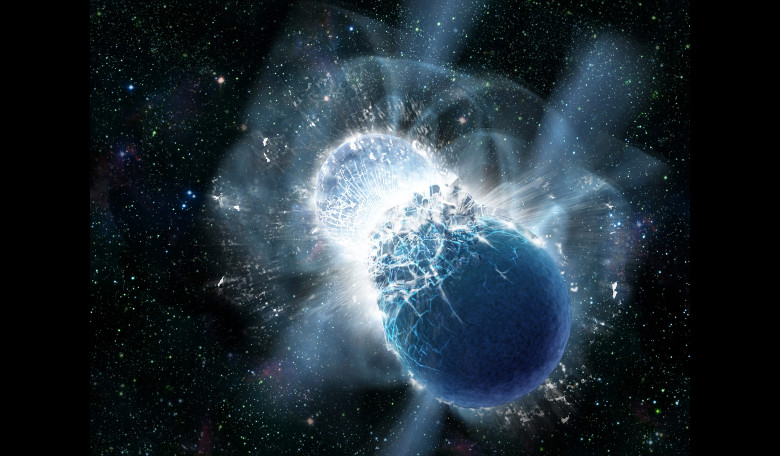
\includegraphics[height=5.5cm]{figs_intro/NeutronStarMergerNew.jpg}};
		}
		% FIG AGN <-> |
		\uncover<1->{  
			\node (img5)[anchor=center,scale=1,opacity=1] at 
			([shift={(-3.5cm, 1.5cm)}]current page.center) {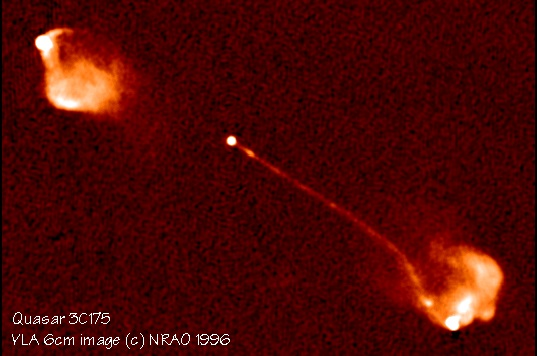
\includegraphics[height=3.5cm]{figs_intro/agn.png}};
		}
		% FIG WR	
		\uncover<2->{  
			\node (img4)[anchor=center,scale=1,opacity=1] at ([shift={(-3.0cm,-2.5cm)}]current page.center) {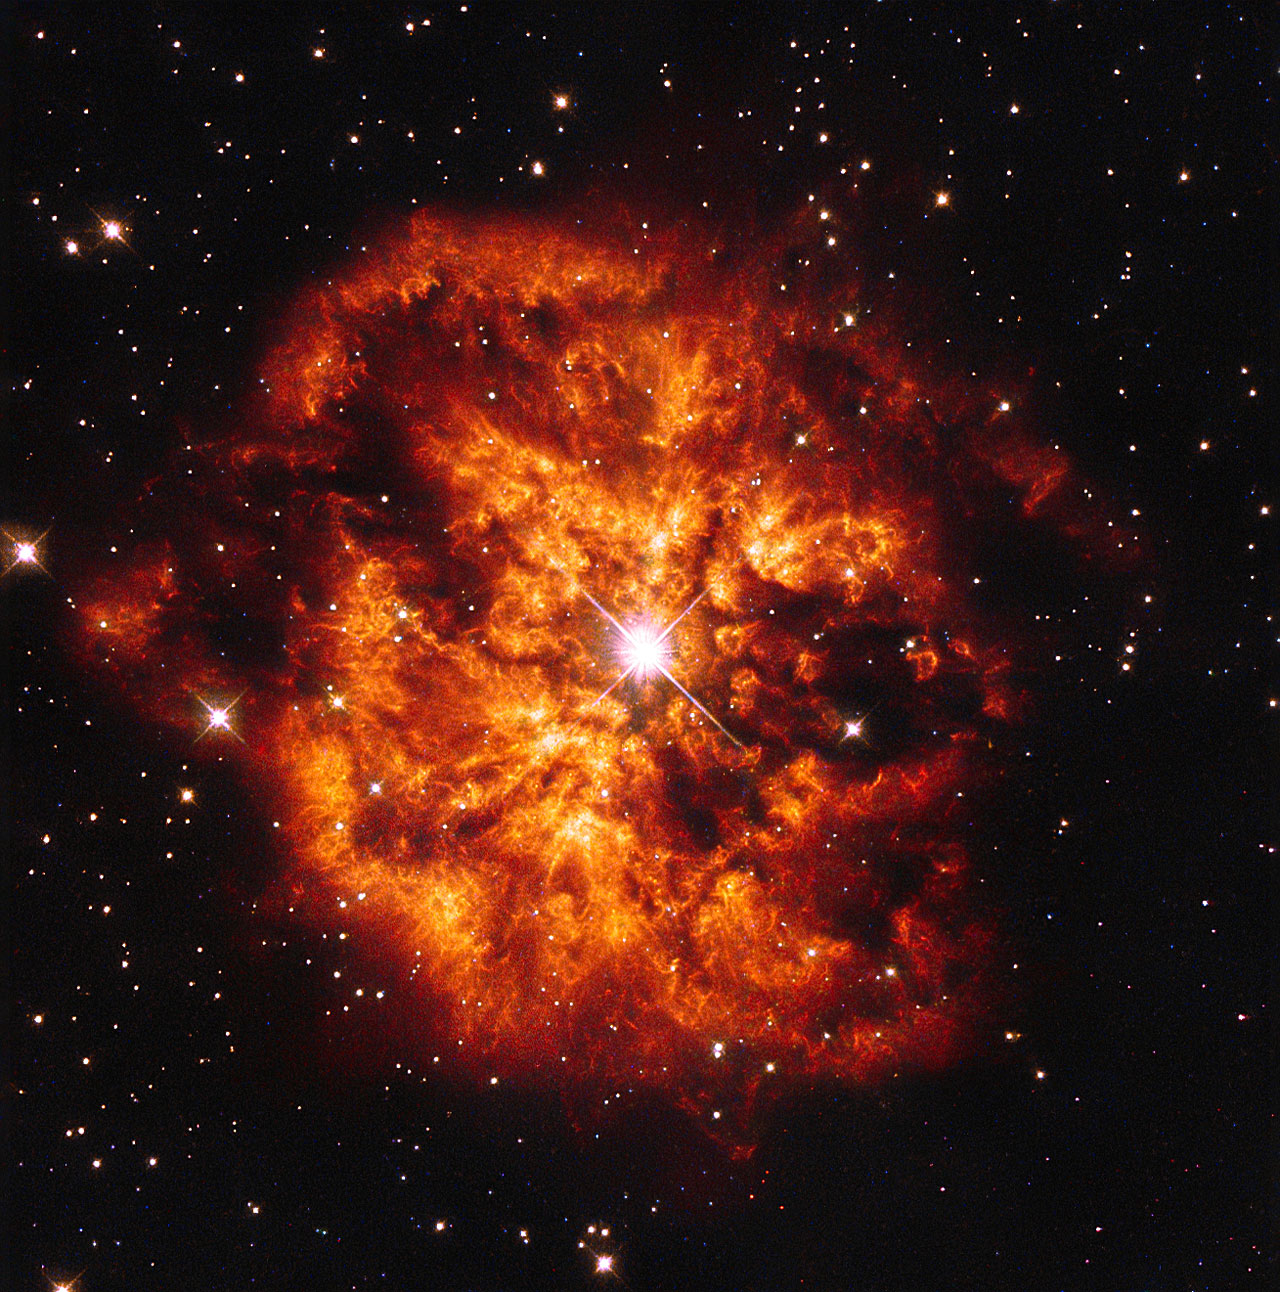
\includegraphics[height=4.5cm]{figs_intro/wr124.jpg}};
		}
		% TEXT 1
		\uncover<3->{  
			\node (t1) [anchor=center,scale=1,opacity=1] at ([shift={(2.8cm,-4.1cm)}]current page.center){
			\parbox{0.7\textwidth}{\tiny{\textcolor{gray}{Sources: \url{https://room.eu.com/contributors/Dr-Kerry-Hebden} \\ 
				\url{https://www.spacetelescope.org/images/potw1533a/} \\
				\url{https://www.britannica.com/science/active-galactic-nucleus}}}
			}};
		}
	\end{tikzpicture} 
\end{frame}

\subsection{Spiral Wave Wind}
\begin{frame}{}
    \begin{tikzpicture}[overlay,remember picture]
    
    \node (t1) [anchor=center,scale=1,opacity=1] at ([shift={(-3.95cm,3.70cm)}]current page.center){
    \parbox{0.4\textwidth}{\tiny{\textcolor{white}{[arXiv:1907.04872]}}
    }};
    
    % SIM NAME | DD2 |
    \uncover<1->{  
    	\node (t1) [anchor=center,scale=1,opacity=1] at 		([shift={(2.8cm,4.10cm)}]current page.center){
    	\parbox{0.8\textwidth}{\scriptsize{\textcolor{black}{DD2 M13641364}
    	}}};
	}
    % D2 MAP | DD2 |
    \uncover<2->{  
    	\node (img1)[anchor=center,scale=1,opacity=1] at ([shift={(0.45cm,1.40cm)}]current page.center) {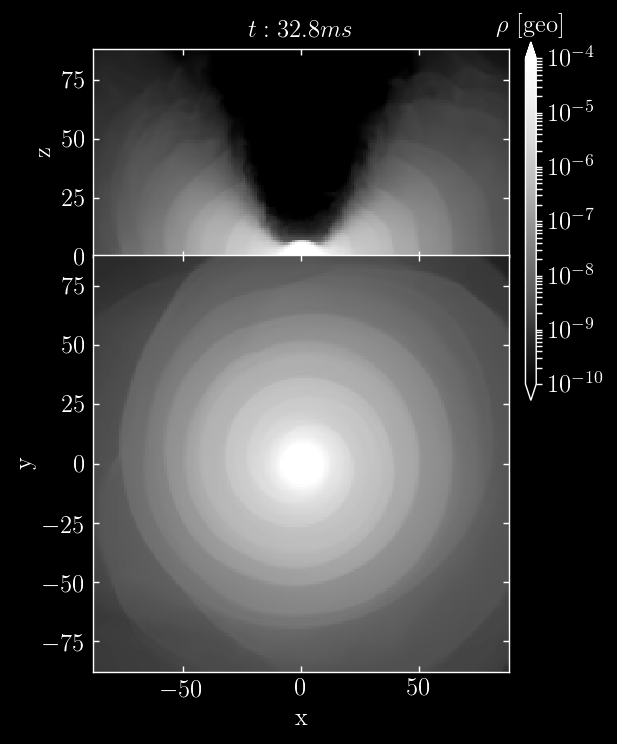
\includegraphics[height=5cm]{figs_dd2/0710656.png}};
    }
    % D2 MAP | LS220 |
    \uncover<3->{  
    	\node (img2)[anchor=center,scale=1,opacity=1] at ([shift={(4.3cm,1.40cm)}]current page.center) {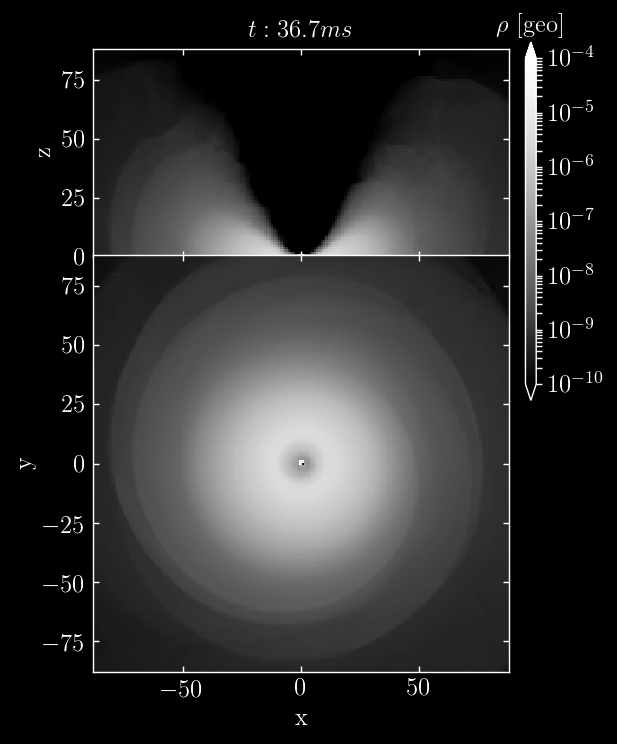
\includegraphics[height=5cm]{figs_ls220/0794624.png}};
    }
    % Cartoon
    \uncover<5->{  
    	\node (img5)[anchor=center,scale=1,opacity=1] at ([shift={(-3.23cm,-2.60cm)}]current page.center) {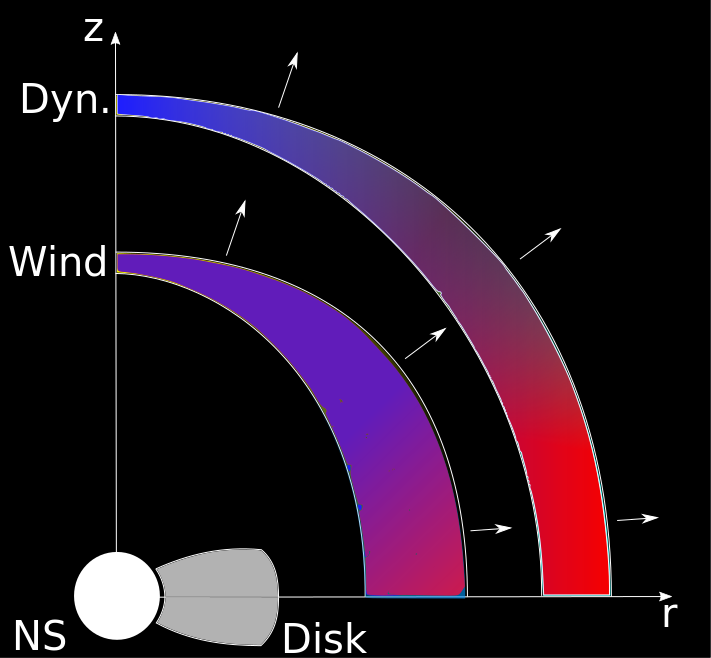
\includegraphics[height=3cm]{figs_cartoon/cart2comp.png}};
    }

    % SIM MAME | LS220 |
    \uncover<2->{  
    	\node (t4) [anchor=center,scale=1,opacity=1] at ([shift={(7.0cm,4.10cm)}]current page.center){
    	\parbox{0.8\textwidth}{\scriptsize{\textcolor{black}{LS220 M13641364}
    	}}};
	}
    % Ejecta | LS220 |
    \uncover<4->{  
    	\node (img3)[anchor=center,scale=1,opacity=1] at ([shift={(3.81cm,-2.60cm)}]current page.center) {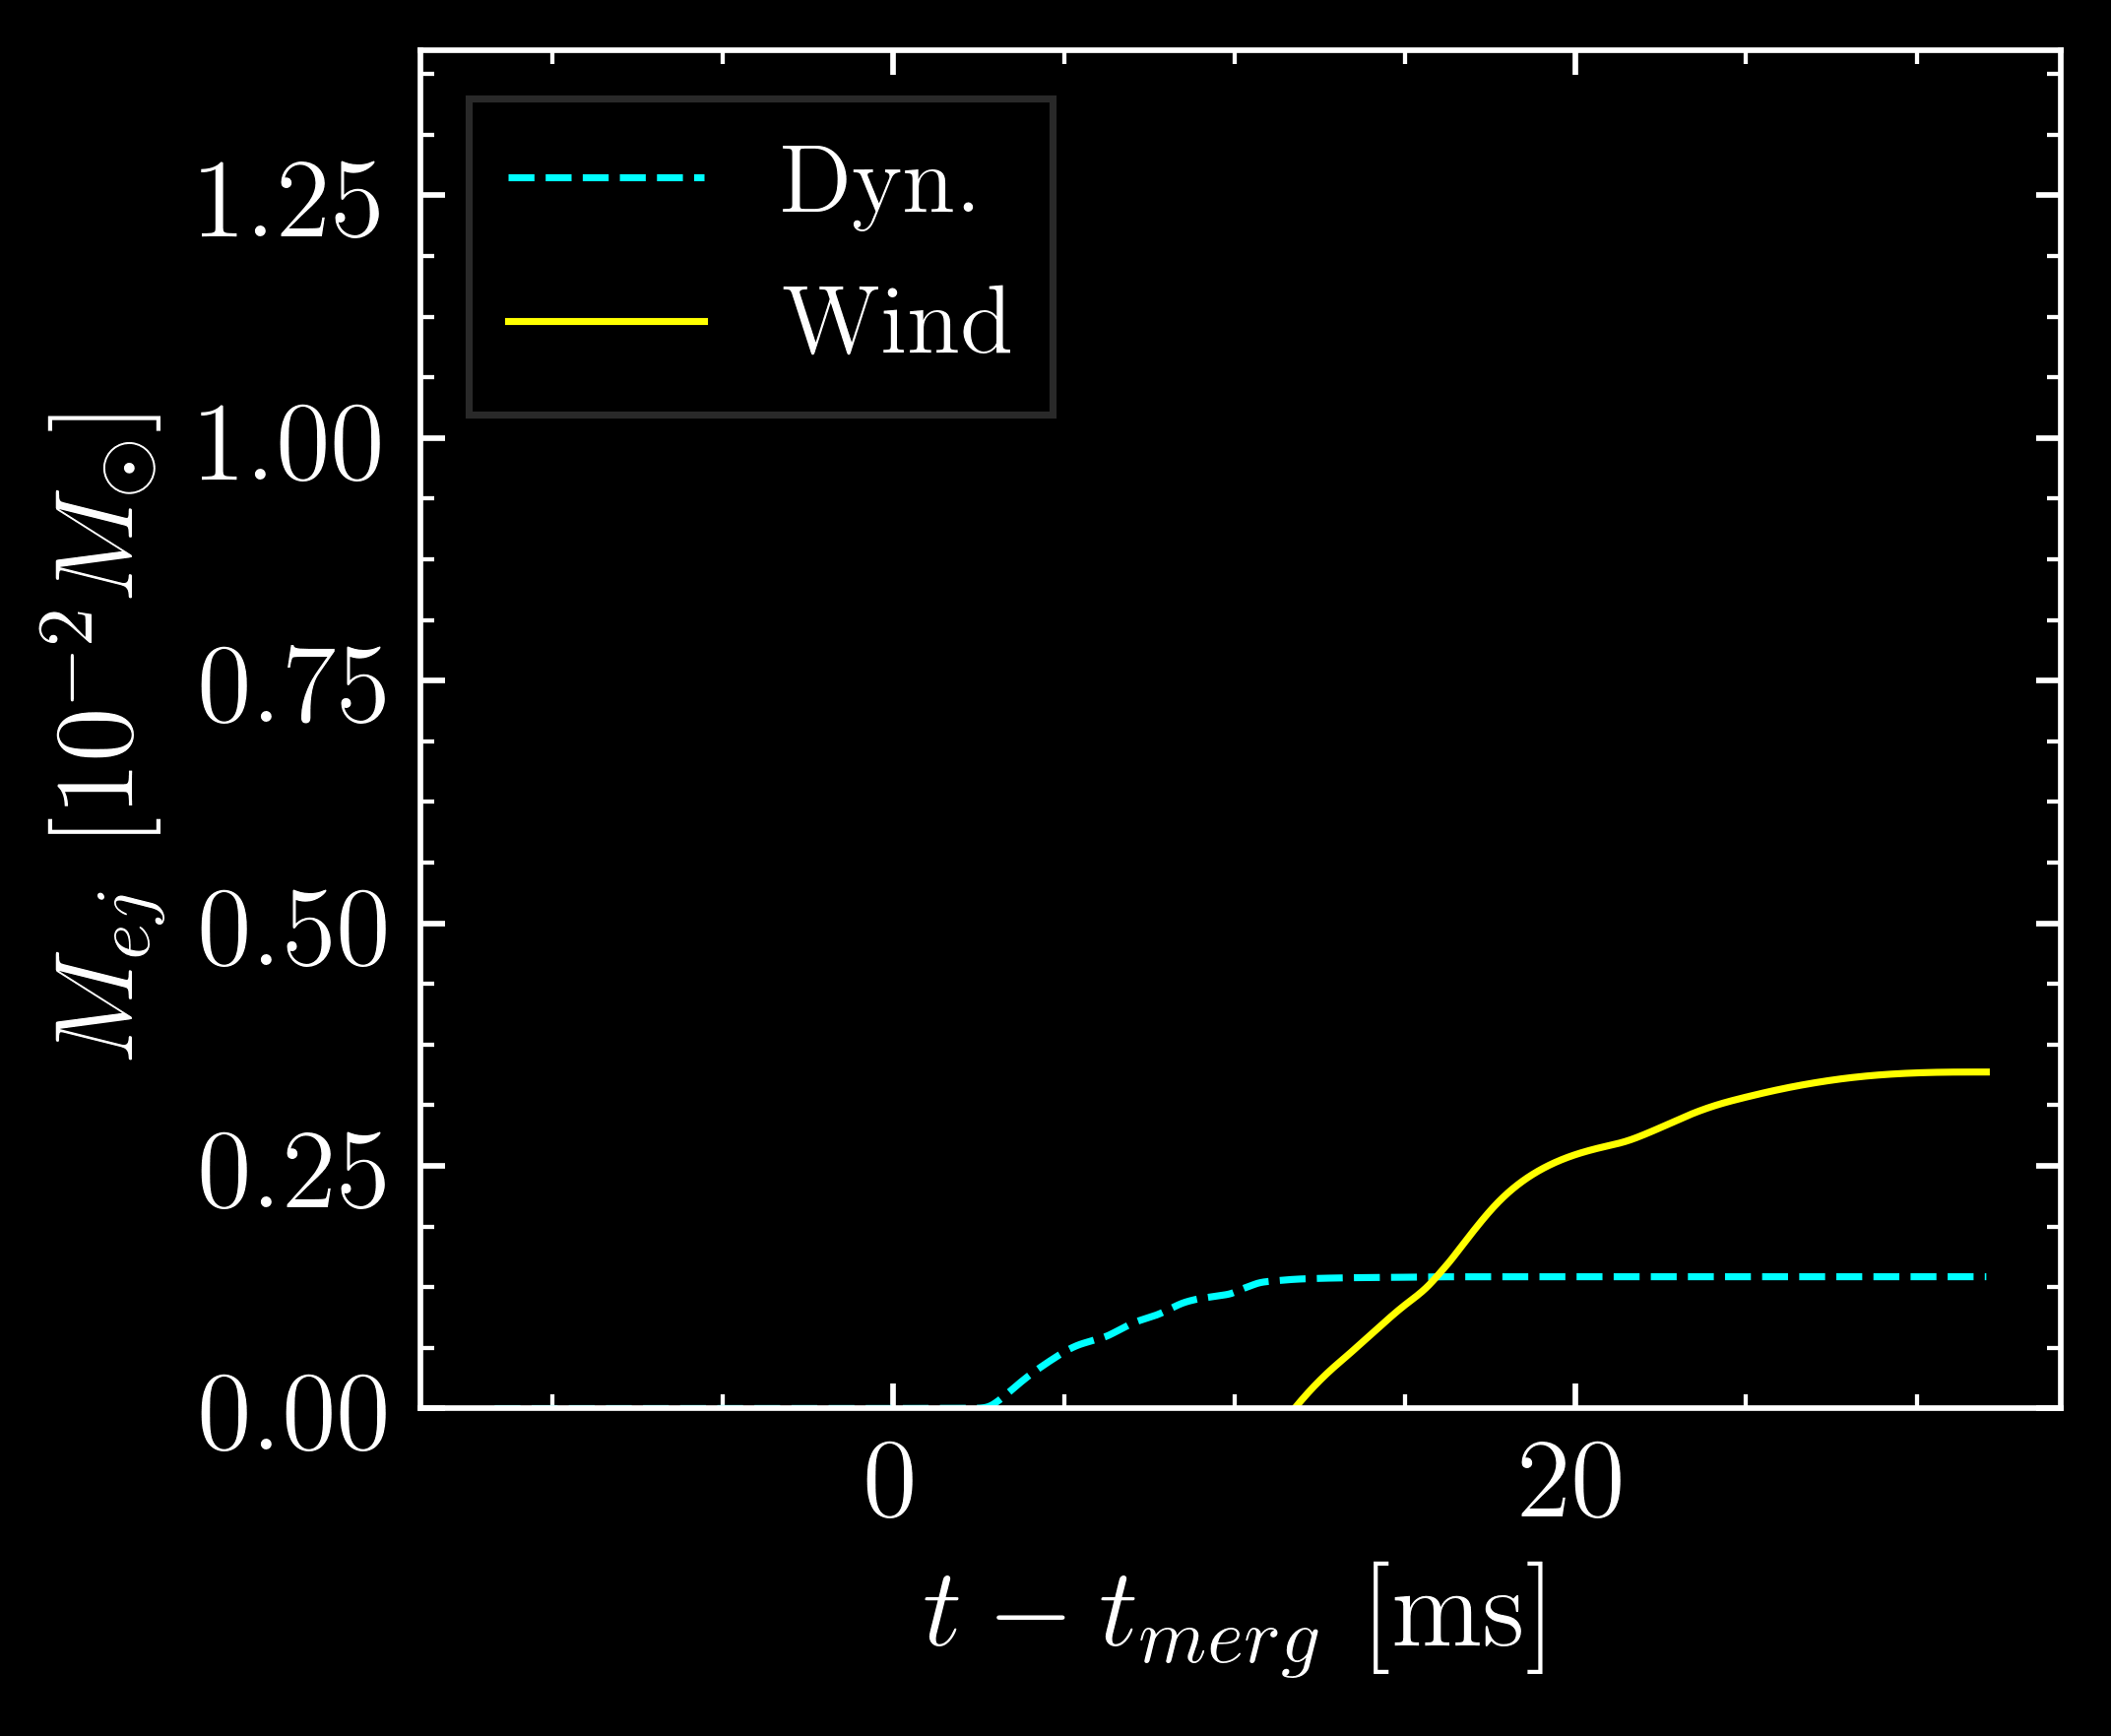
\includegraphics[height=3cm]{figs_ls220/ejecta_profile_dyn_bern.png}};
    }
	% Ejecta | DD2 | 
    \uncover<4->{  
    	\node (img4)[anchor=center,scale=1,opacity=1] at ([shift={(0.20cm,-2.60cm)}]current page.center) {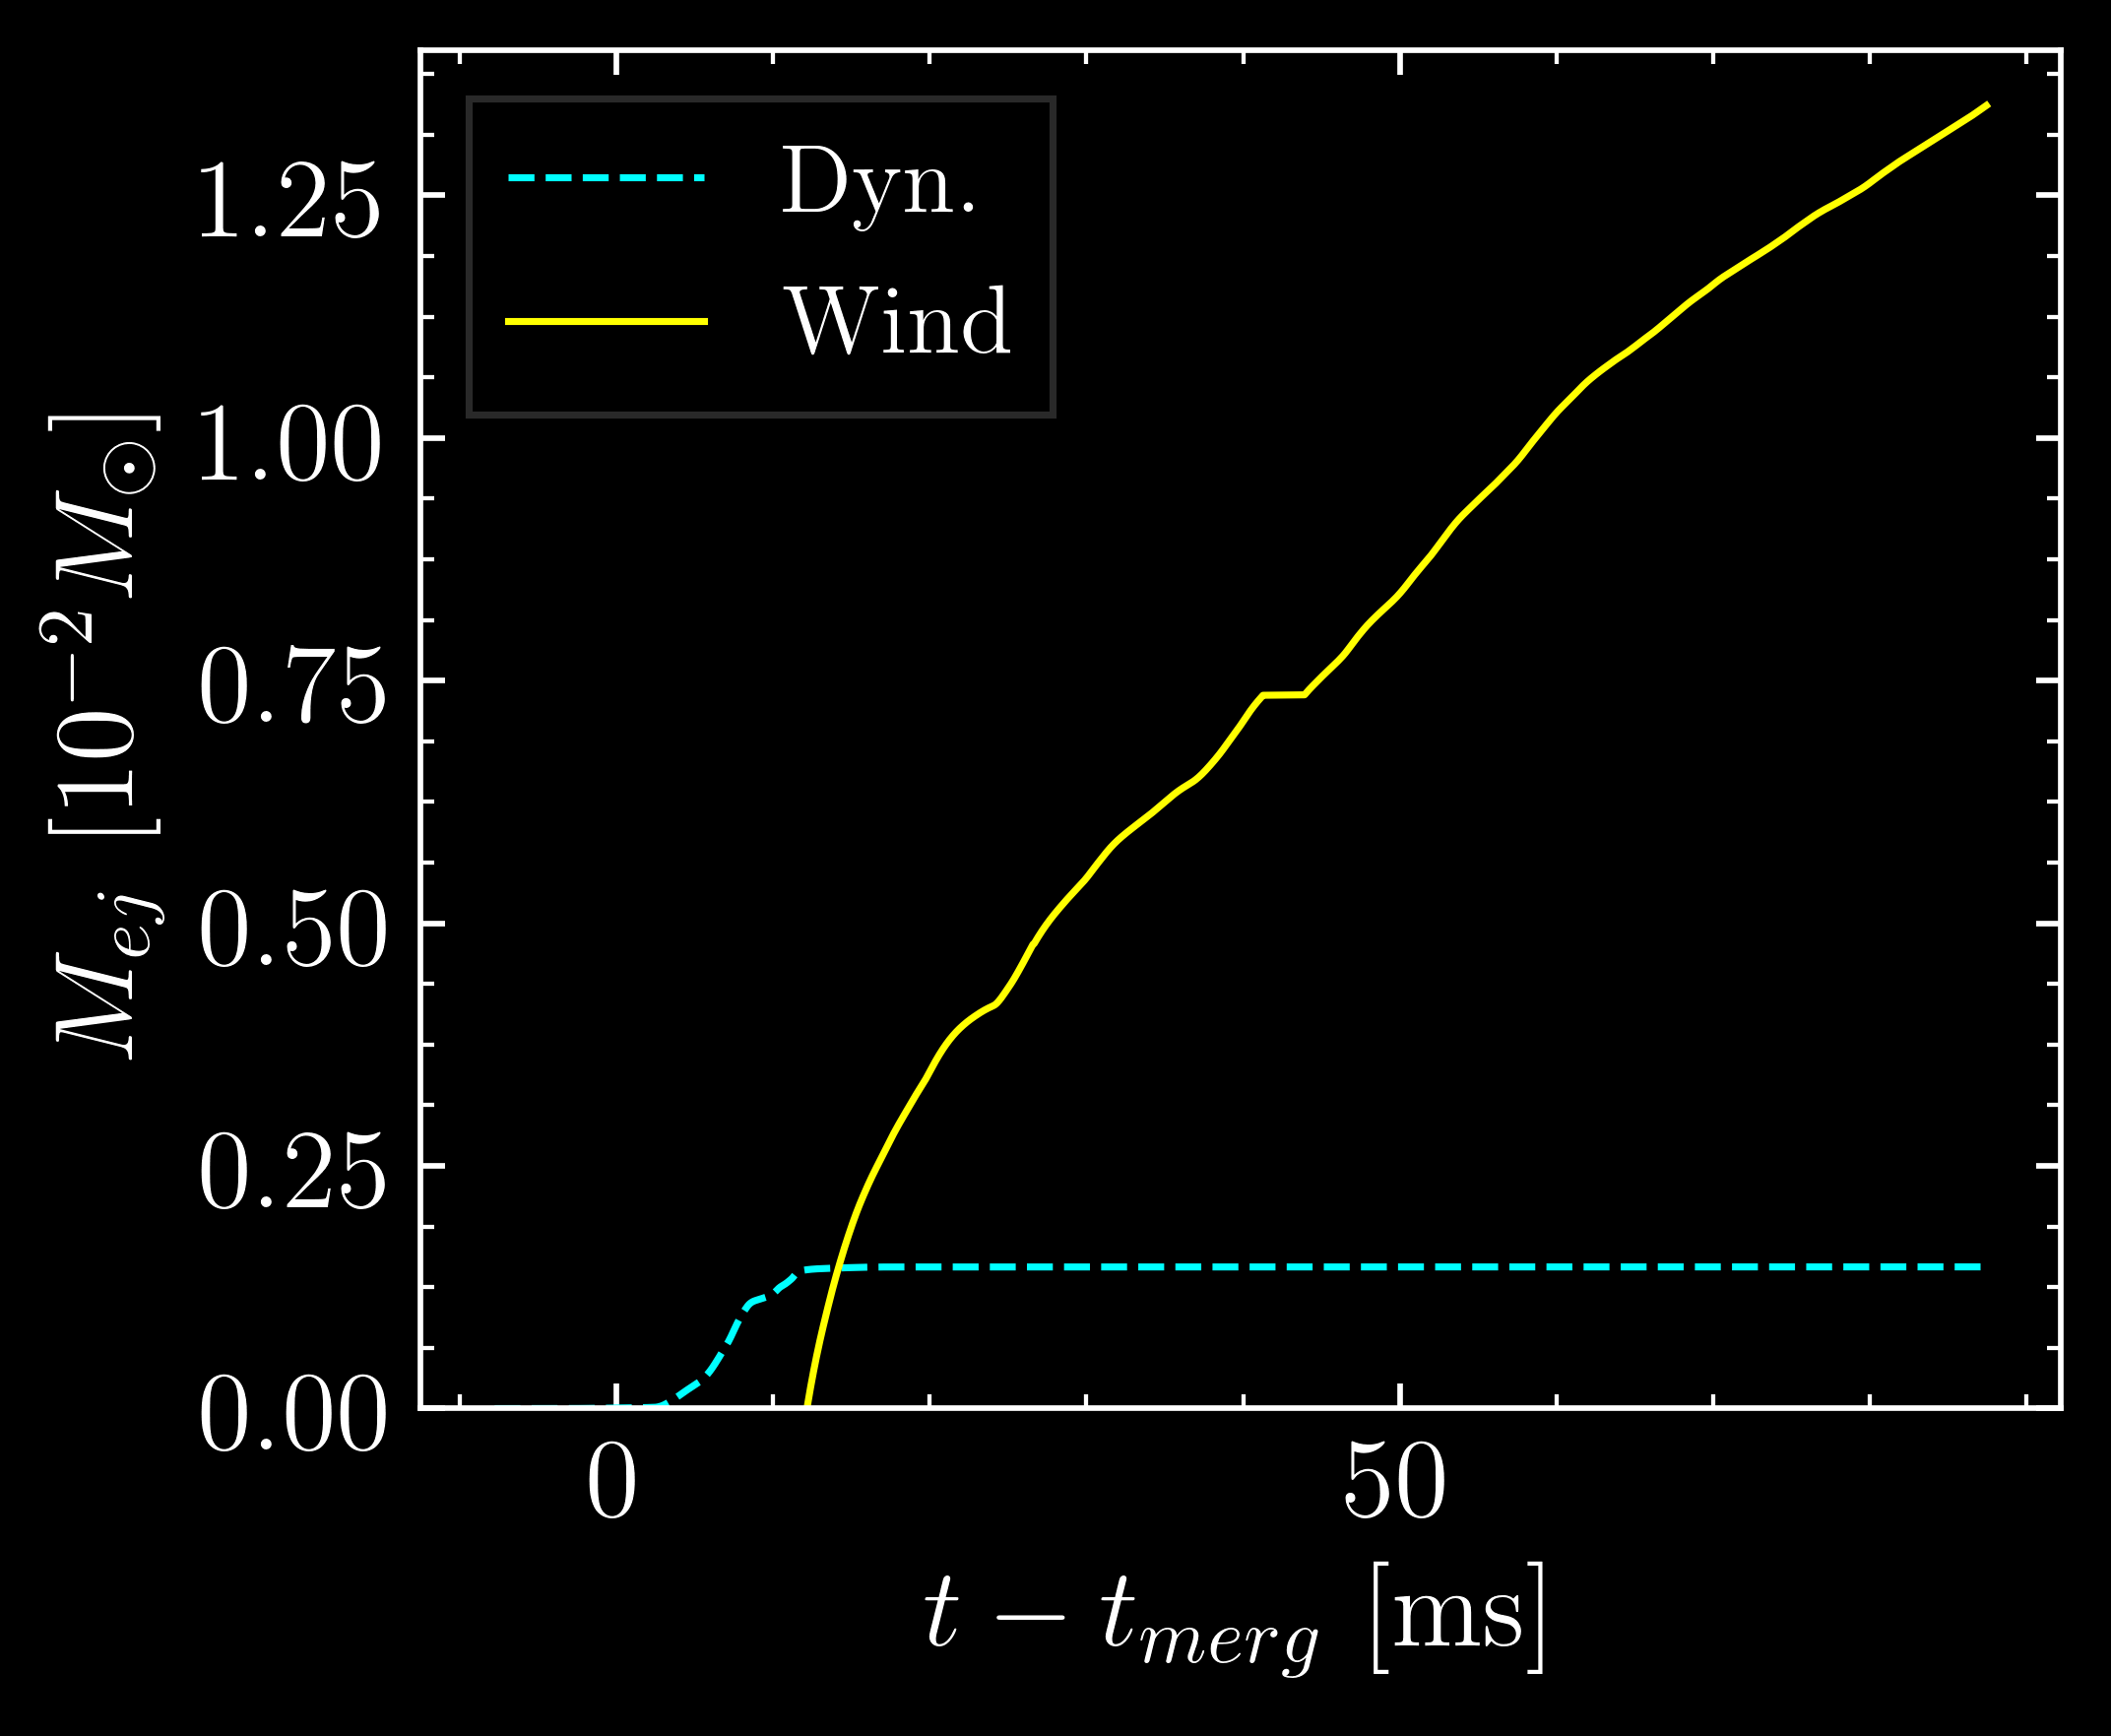
\includegraphics[height=3cm]{figs_dd2/ejecta_profile_dyn_bern.png}};
    }
    % MKN 
    
    \uncover<6->{    
        \node (img5)[anchor=center,scale=1,opacity=1] at ([shift={(-3.95cm,0.75cm)}]current page.center) {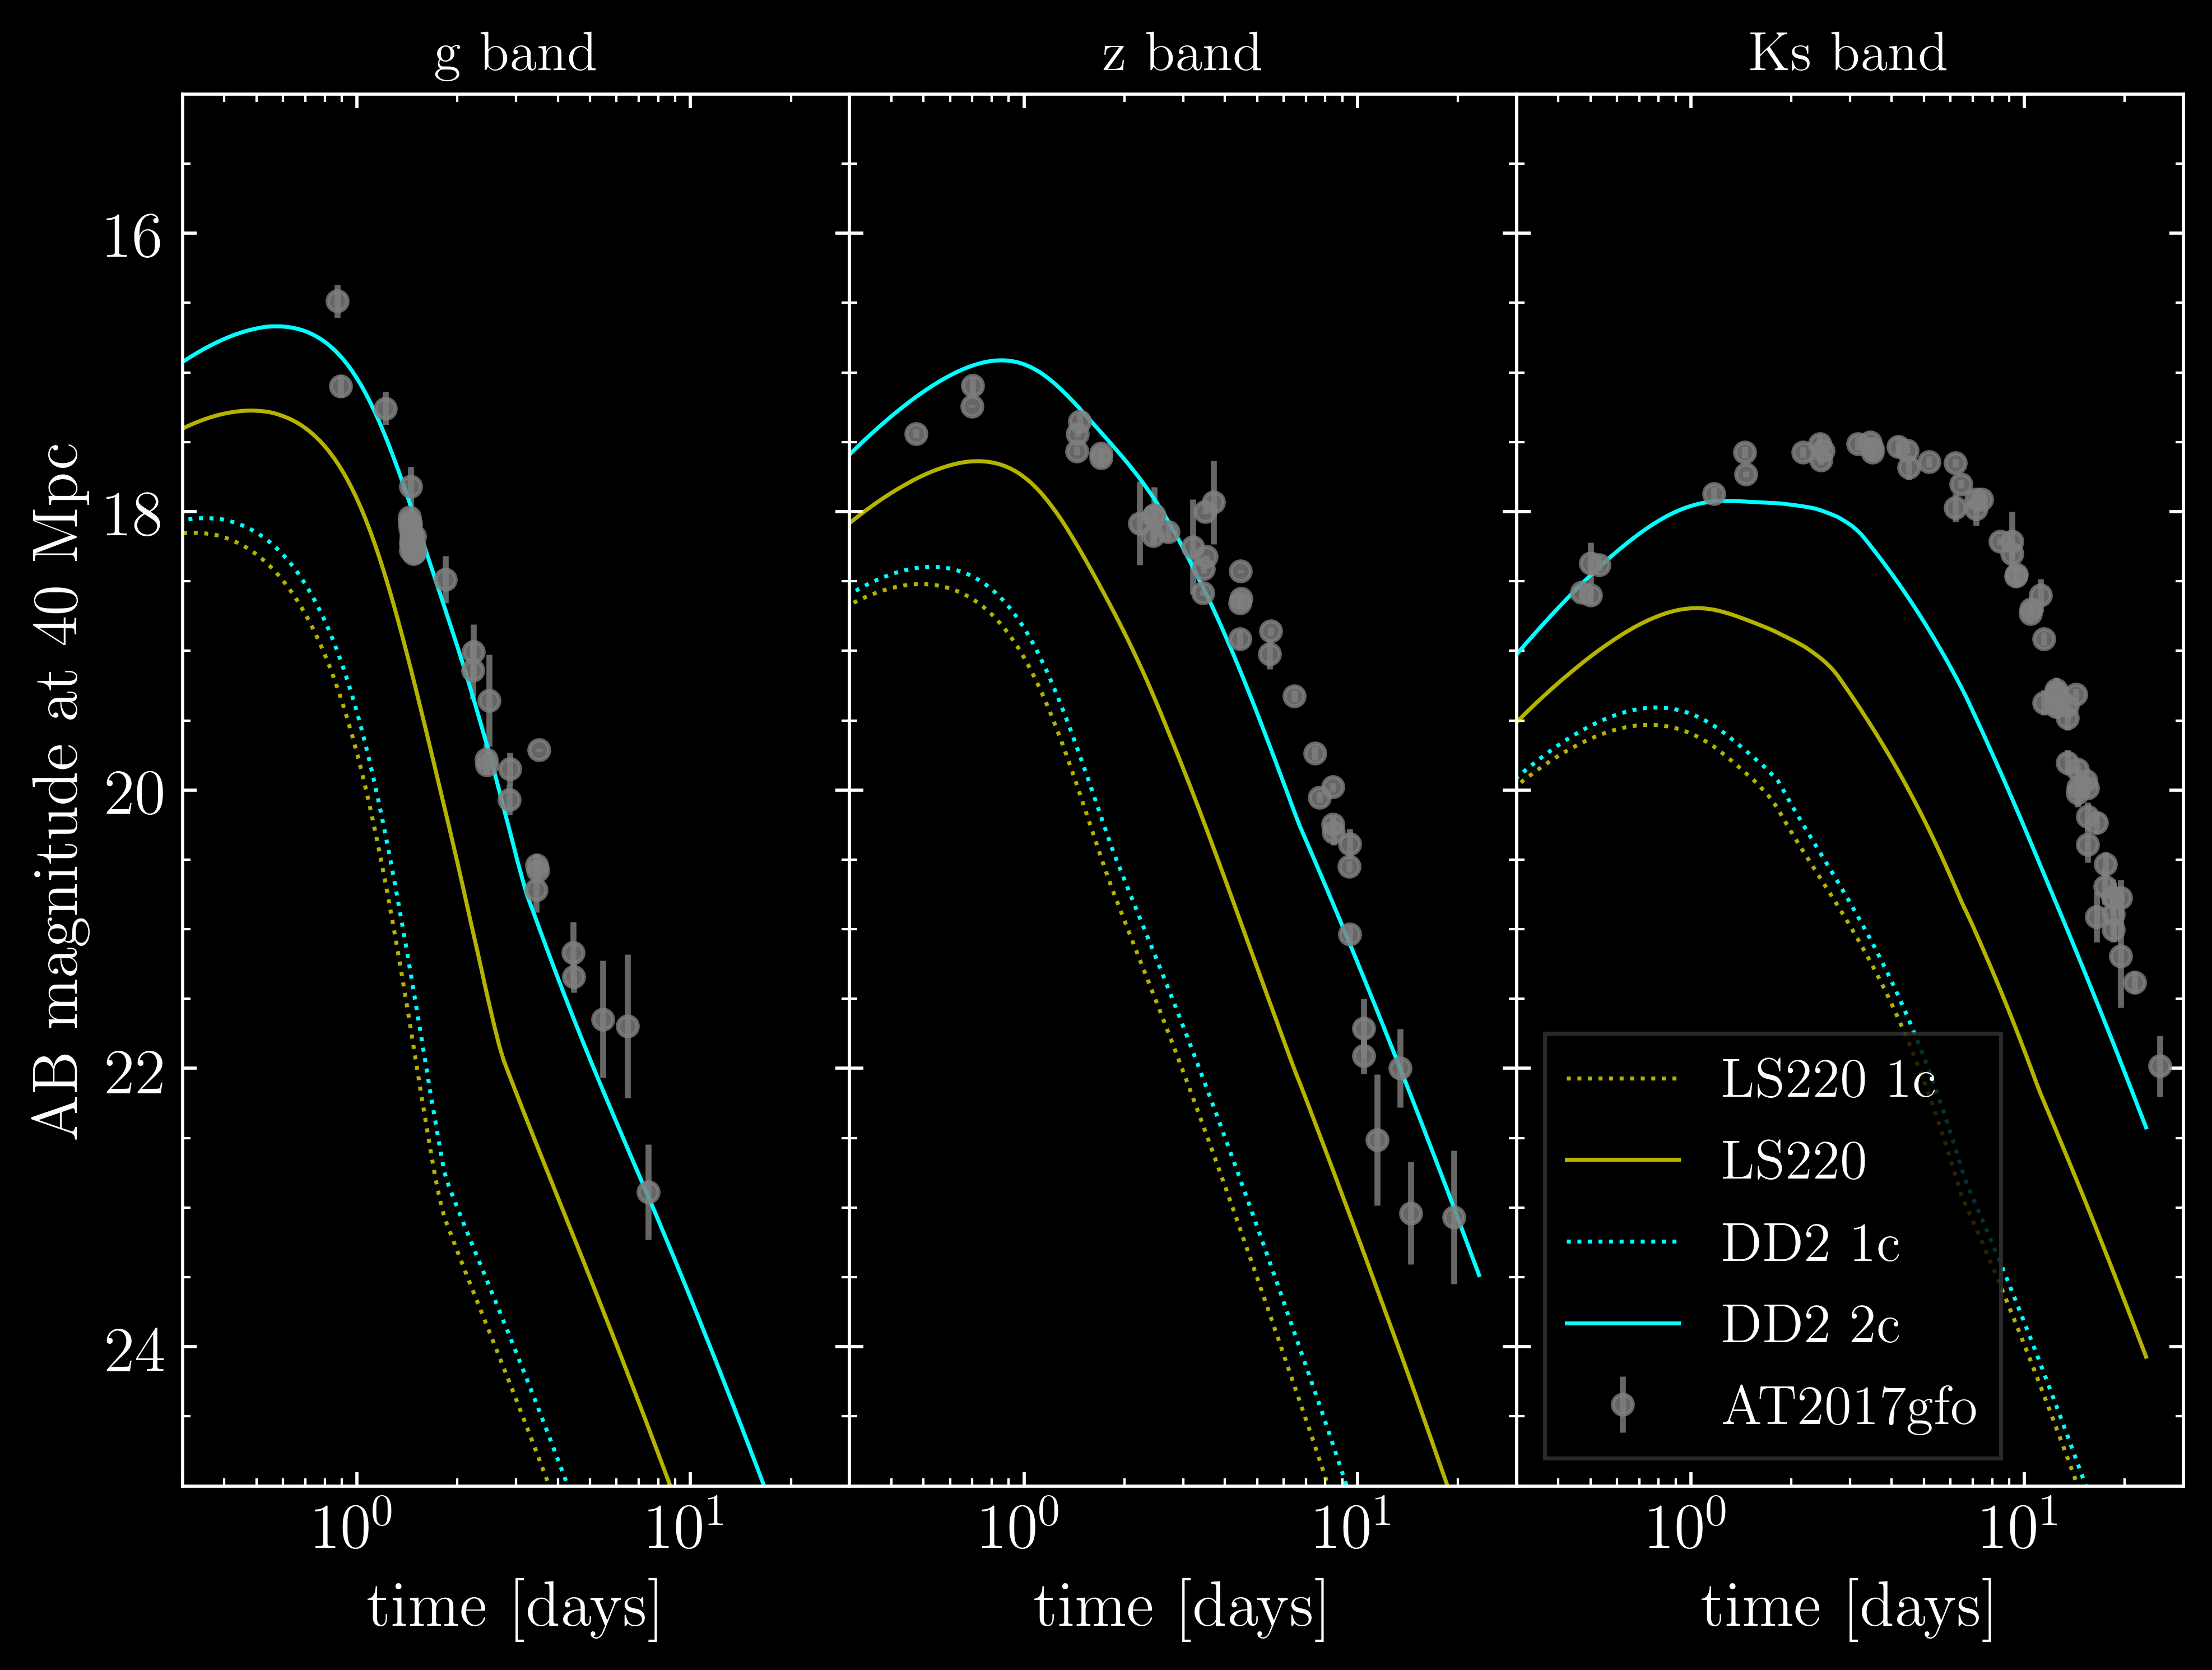
\includegraphics[height=3.7cm]{figs_mkn/mkn2comp.png}};
    }

    \end{tikzpicture} 
\end{frame}


\end{document}
